%%% Econ712: Macroeconomics I
%%% Fall 2020
%%% Danny Edgel
%%%
% Due on Canvas Thursday November 19th, 11:59pm Central Time
%%%

%%%
%							PREAMBLE
%%%

\documentclass{article}

%%% declare packages
\usepackage{amsmath}
\usepackage{amssymb}
\usepackage{array}
\usepackage{bm}
\usepackage{changepage}
\usepackage{centernot}
\usepackage{graphicx}
\usepackage[shortlabels]{enumitem}
\usepackage{fancyhdr}
	\fancyhf{} % sets both header and footer to nothing
	\renewcommand{\headrulewidth}{0pt}
    \rfoot{Edgel, \thepage}
    \pagestyle{fancy}
	
%%% define shortcuts for set notation
\newcommand{\N}{\mathbb{N}}
\newcommand{\Z}{\mathbb{Z}}
\newcommand{\R}{\mathbb{R}}
\newcommand{\Q}{\mathbb{Q}}
\newcommand{\lmt}{\underset{x\rightarrow\infty}{\text{lim }}}
\newcommand{\neglmt}{\underset{x\rightarrow-\infty}{\text{lim }}}
\newcommand{\zerolmt}{\underset{x\rightarrow 0}{\text{lim }}}
\newcommand{\loge}[1]{\text{ln}\left(#1\right)}
\newcommand{\usmax}[1]{\underset{#1}{\text{max }}}
\newcommand{\Mt}{M_{t+1}^t}
\newcommand{\vhat}{\hat{v}}
\newcommand{\olp}{\overline{p}}
\renewcommand{\L}{\mathcal{L}}
\newcommand{\olq}{\overline{q}}
\newcommand{\zinf}{_{t=0}^\infty}
\newcommand{\aneg}{A^{-1}}
\newcommand{\sneg}{s^{-1}}
\newcommand{\olk}{\overline{k}}
\newcommand{\olc}{\overline{c}}
\newcommand{\olr}{\overline{r}}
\newcommand{\olpi}{\overline{\pi}}
\newcommand{\Aneg}{A^{-1}}
\renewcommand{\sneg}{s^{-1}}

\DeclareMathOperator{\E}{\mathbb{E}} % expected value

%%% define column vector command (from Michael Nattinger)
\newcount\colveccount
\newcommand*\colvec[1]{
        \global\colveccount#1
        \begin{pmatrix}
        \colvecnext
}
\def\colvecnext#1{
        #1
        \global\advance\colveccount-1
        \ifnum\colveccount>0
                \\
                \expandafter\colvecnext
        \else
                \end{pmatrix}
        \fi
}

%%% define function for drawing matrix augmentation lines
\newcommand\aug{\fboxsep=-\fboxrule\!\!\!\fbox{\strut}\!\!\!}

\makeatletter
\let\amsmath@bigm\bigm

\renewcommand{\bigm}[1]{%
  \ifcsname fenced@\string#1\endcsname
    \expandafter\@firstoftwo
  \else
    \expandafter\@secondoftwo
  \fi
  {\expandafter\amsmath@bigm\csname fenced@\string#1\endcsname}%
  {\amsmath@bigm#1}%
}


%________________________________________________________________%

\begin{document}

\title{	Problem Set \#2 }
\author{ 	Danny Edgel 					\\ 
			Econ 712: Macroeconomics I		\\
			Fall 2020						\\
		}
\maketitle\thispagestyle{empty}

%%%________________________________________________________________%%%

\noindent\textit{Collaborated with Sarah Bass, Emily Case, Michael Nattinger, and Alex Von Hafften}

%%%________________________________________________________________%%%
\subsection*{Question 1}

\begin{enumerate}[(a)]
	\item In a balanced growth path, households' utility and firms' profits are maximized. Thus, to find a system of equations that $C_0$, $N_0$, $w_0$, and $r_0$ must solve in a balanced growth path, we must characterize and solve the household and firm problems. To start, the household problem is given by 
		\[
			\usmax{\left\{C_t,K^s_{t+1},N^s_t\right\}_{t=0}^\infty}\sum_{t=0}^\infty \beta_t u(C_t,1-N_t)\text{ s.t. }
				\sum_{t=0}^\infty p_t\left(C_t + K_{t+1}\right) \leq \sum_{t=0}^\infty p_t\left(r_tK_t + W_tN_t\right) + \pi_0
		\]
		And the firm's problem is:
		\[
			\usmax{\left\{K_t^d,N_t^d\right\}_{t=0}^\infty}\pi_0 = \sum\zinf p_t\left(Y_t-r_tK_t^d - W_tN_t^d\right)\text{ s.t. } Y_t\leq F(K_t^d,A_tN_t^d)
		\]
		Where, recognizing that $\pi_0$ is monotone in $Y_t$, the firm's problem can be reduced to:
		\[
			\usmax{\left\{K_t^d,N_t^d\right\}_{t=0}^\infty}\pi_0 = \sum\zinf p_t\left(F(K_t^d,A_tN_t^d)-r_tK_t^d - W_tN_t^d\right)
		\]
		Since the firm is a price-taker whose decision in each period has no bearing on its conditions in any other period, the firm's problem can be solved by solving a single arbitrary period, $t$, using first-order conditions. For all choice variables, $X$, let ${\frac{X_t}{A_t} = x_t}$:
		\[
			\usmax{\left\{k_t^d,N_t^d\right\}_{t=0}^\infty}\pi_0 = \sum\zinf A_tp_t\left(F(k_t^d,N_t^d)-r_tk_t^d - w_tN_t^d\right)
		\]
		\begin{align*}
			&K_t^d: & A_tp_tF_K(k_t^d,N_t^d) -A_tp_tr_t = 0	\\
			&		& F_K(k_t^d,N_t^d) = r_t				\\
			&N_t^d:	& p_tF_N(k_t^d,N_t^d) -p_tw_t = 0	\\
			&		& F_N(k_t^d,N_t^d) = w_t
		\end{align*}
		This solution ensures that that $\pi_0=0$. Assuming that the utility function is concave, strictly increasing, and differentiable, the constrating of the household problem holds with equality and an interior solution exists. Given the firm's solution, we can solve the constraint as:
		\[
				c_t = (r_t+1-\delta)k^s_t + w_tN^s_t - k^s_{t+1}
		\]
		Such that the household's problem has the Lagrangian function:
		\[
			\L = \sum\zinf\left[\beta^tu(A_tc_t,N_t) - p_t\lambda\left(c_t + k_{t+1} - (r_t+1-\delta)k_t - w_tN_t\right)\right]
		\]
		Which has the first-order conditions:
		\begin{align*}
			&c_t: 			& \beta^tA_tu_c(A_tc_t,N_t) = 	p_t\lambda 									\\
			&c_{t+1}:		& \beta^{t+1}A_{t+1}u_c(A_{t+1}c_{t+1},N_{t+1}) = 	p_{t+1}\lambda 			\\
			&N_t:			& -\beta^t\frac{u_N(A_tc_t,N_t)}{w_t} = p_t\lambda							\\
			&N_{t+1}:		& \beta^{t+1}\frac{-u_N(A_{t+1}c_{t+1},N_{t+1})}{w_{t+1}} = p_{t+1}\lambda	\\
			&k_{t+1}:		& \frac{p_t}{p_{t+1}} = r_{t+1} + 1 - \delta
		\end{align*}
		Where the growth of households' optimal level of consumption is dependent on wage growth:
		\[
			-u_N(A_tc_t,N_t)/w_t = A_tu_c(A_tc_t,N_t) 
		\]
		
		In equilibrium, all markets clear:
		\begin{align*}
			K_t^s &= K_t^d									&\text{(Capital)}	\\
			N_t^s &= N_t^d 									&\text{(Labor)}		\\
			C_t + K_{t+1} - (1-\delta)K_t &= F(K_t,A_tN_t)	&\text{(Goods)}
		\end{align*}
		And each initial choice variable, $N_0$ and $C_0$, and price, $w_0$ and $r_0$, satisfies the firm and household optimization conditions for a balanced growth path:
		\begin{align*}
			F_K(k_0,N_0) &= r_0									\\
			F_N(k_0,N_0) &= w_0									\\
			-\frac{u_N(A_0c_0,N_0)}{u_c(A_0c_0,N_0)} &= w_0A_0	\\
			c_0 + k_{1} - (1-\delta)K_0 &= F(k_0,N_0)
		\end{align*}
	
	\item Let $u(C,N) = \frac{C^{1-\gamma}}{1-\gamma}h(1-N)$, where $\gamma>0$, $\gamma\neq 1$. Then, the first-order conditions, provided in (a), can be used to derive:
		\begin{align}
			\beta(1+g)^{1-\gamma}\left(\frac{c_{t+1}}{c_t}\right)^{-\gamma}\left(\frac{h(1-N_{t+1})}{h(1-N_t)}\right) &= \frac{p_{t+1}}{p_t}	\\
			\beta(1+g)^{1-\gamma}\left(\frac{c_{t+1}}{c_t}\right)^{1-\gamma}\left(\frac{h'(1-N_{t+1})}{h'(1-N_t)}\right) &= \left(\frac{w_{t+1}}{w_t}\right)\left(\frac{p_{t+1}}{p_t}\right)	\\
			r_{t+1} + 1 - \delta &= \frac{p_t}{p_{t+1}}
		\end{align}
		In a balanced growth path, capital is rented at a constant $\overline{r}$. Thus, by equation (3), the price level grows at constant rate $\overline{\pi}$:
			\[
				\overline{\pi} = \frac{1}{\overline{r} + 1 - \delta}
			\]
		Further, in a balanced growth path, ${N_t=N_{t+1}=\overline{N}}$. Thus, equations (1) and (2) become:
		\begin{align}
			\beta(1+g)^{1-\gamma}\left(\frac{c_{t+1}}{c_t}\right)^{-\gamma} &= \overline{\pi}	\\
			\beta(1+g)^{1-\gamma}\left(\frac{c_{t+1}}{c_t}\right)^{1-\gamma} &= \left(\frac{w_{t+1}}{w_t}\right)\overline{\pi}
		\end{align}
		By dividing (5) by (4), solve for the wage growth rate:
		\[
			\frac{c_{t+1}}{c_t} = \frac{w_{t+1}}{w_t}
		\]
		So consumption growth is equal to wage growth. In a balanced growth path, standardized variables (those scaled by $A_t$) are stationary, so we can solve for $\overline{pi}$ and $\overline{r}$ using (4):
		\begin{align*}
			\beta(1+g)^{1-\gamma} &= \overline{\pi}	\\
			(\overline{r} + 1 - \delta)\beta(1+g)^{1-\gamma} &= 1	\\
			\overline{r} &= \frac{1 - (1-\delta)\beta(1+g)^{1-\gamma}}{\beta(1+g)^{1-\gamma}}
		\end{align*}
		Knowing that, when scaled by $A_t$, capital, consumption, and output will all be constant, we can also solve for those values using the law of motion:
		\[
			\overline{c} + (g+\delta)\overline{k} = F(\overline{k},\overline{N})
		\]
		Thus, there will be a balanced growth path for $\gamma >0$, $\gamma\neq 1$. For $\gamma=1$, we can see that the first-order conditions will yield the same result, but with a different inflation (and thus interest) rate:
		\begin{align*}
			\beta(1+g)\left(\frac{c_t}{c_{t+1}}\right) &= \overline{\pi}	\\
			\beta\left(\frac{h'(1-N_{t+1})}{h'(1-N_{t+1})}\right) &= \left(\frac{w_{t+1}}{w_t}\right)\overline{\pi}
		\end{align*}
		
	\item We cannot characterize this system with a phase diagram because the optimal level of capital and consumption depend not only on each other, but also on labor supply, which adds a third dimension to the system. Since we don't know the specific relationship between labor supply and utility, we cannot say whether an increase in, say, $\delta$, will ultimately lead to a higher or lower level of consumption and capital because a higher marginal rate of substitution (MRS) of consumption for liesure could lead to greater consumption, while a lower MRS could lead to higher liesure levels but lower capital and consumption.
	
	\item If $h$ is a constant function, then, since liesure is not valued, $N_t=1$ for all $t$, and, letting ${F(k,1)=f(k)}$, each of the system's variables can be solved by equations with known parameterized values:
		\begin{align*}
			& \overline{\pi}	= \beta(1+g)^{1-\gamma}						&\text{(consumption FOC)} 		\\
			& \overline{r}   	= \frac{1}{\overline{\pi}} - (1 - \delta)	&\text{(capital  FOC)} 			\\
			& \overline{w} 		= f(\overline{k}) -\overline{r}\overline{k}	&\text{(zero profit)} 			\\
			& \overline{k} 		= f'(f^{-1}(\overline{r}))					&\text{(firm FOC)}				\\
			& \overline{c} 		= f(\overline{k}) - (g+\delta)\overline{k}	&\text{(law of motion)}		 	\\
			& \overline{y} 		= f(\overline{k}) 							&\text{(production function)}	
		\end{align*}
	
	\item Suppose there is a decrease in the rate of technology, $g$. This causes a decrease in the rate of inflation, $\overline{pi}$, which increases the interest rate, $\overline{r}$. Long-run $\overline{k}$ is equal to the derivative of the production function at the inverse of the production function at $\overline{r}$. Since $f$ is increasing but concave, an increase in $\overline{r}$ causes a decrease in the long-run value of $\overline{k}$.
	
	Now consider the effect on consumption. A decrease in $\overline{k}$ causes a decrease in $\overline{k}$ but decreases $(g+\delta)\overline{k}$ (which is also shrunk by the first-order effect of a decrease in $g$). Thus, the effect of $g$'s decrease in consumption in the long term depends on the specification of $f$.
	
	In the short run, capital levels are fixed. Thus, in order to move from the initial steady state to the new steady state, consumption will spike, followed by a gradual decrease in both $c$ and $k$ until the new steady state is reached.
	
	\pagebreak
	\item Define $\overline{s}$ as the gross output that is invested in capital in the steady state and $\overline{\theta}$ be the fraction of output saved. Then, using the law of motion, we can solve,
		\begin{align*}
			\overline{s} 	&= f(\overline{k}) - \overline{c}	\\
			\overline{\theta} &= \frac{\overline{s}}{f(\overline{k}} 	\\
							&= 1-\frac{\overline{c}}{f(\overline{k}}	\\
			\frac{\partial\overline{\theta}}{\partial g} &= -\frac{f(\overline{k})\frac{\partial\overline{c}}{\partial g}-\overline{c}f'(\overline{k})\frac{\partial\overline{k}}{\partial g}}{f(\overline{k})^2}	\\
			\frac{\partial\olc}{\partial g} &= f'(\olk)\frac{\partial\olk}{\partial g} - \frac{\partial\olk}{\partial g}	\\
			\frac{\partial\olk}{\partial g} &= \left(\frac{f''(f^{-1}(\olr))}{f'(f^{-1}(\olr))}\right)\frac{\partial\olr}{\partial g}	\\
			\frac{\partial\olr}{\partial g} &= -\frac{1}{\olpi}\left(\frac{\partial\olpi}{\partial g}\right)	\\
			\frac{\partial\olpi}{\partial g} &= (1-\gamma)\beta(1+g)^{-\gamma}	\\
\Rightarrow	\frac{\partial\overline{\theta}}{\partial g} &= \left(\frac{\partial\overline{k}}{\partial g}\right)\frac{\overline{c}f'(\overline{k})-f(\overline{k})(f'(\overline{k})-1)}{f(\overline{k})^2} 	\\
					&= \left(\frac{f''(f^{-1}(\olr))}{f'(f^{-1}(\olr))}\right)\left(\frac{(\gamma-1)\beta(1+g)^{-\gamma}}{\olpi^2}\right)\frac{\overline{c}f'(\overline{k})-f(\overline{k})(f'(\overline{k})-1)}{f(\overline{k})^2}	\\
					&= \left(\frac{f''(f^{-1}(\olr))}{f'(f^{-1}(\olr))}\right)\left(\frac{(\gamma-1)\beta(1+g)^{-\gamma}}{\olpi^2}\right)\frac{f'(\olk)\left(\overline{c}-f(\olk) + \frac{f(\olk)}{f'(\olk)}\right)}{f(\overline{k})^2}
		\end{align*}
		So the change in fraction of output saved, with respect to $g$, comes down to a product of three terms. Recall that $\gamma>1$ and $f$ is strictly increasing and concave. Thus, the first term is negative and the second term is positive. Further, since savings are always positive, ${\olc<f(\olk)}$, so the third term is negative. Therefore, the overall product is positive, and we can conclude that the fraction of output saved increases when $g$ increases.
		\medskip \\
		Specialzed to Cobb-Douglas production, ${f(k)=k^\alpha}$, so the derivative from above is:
		\[
			\frac{\partial\overline{\theta}}{\partial g} = \left((\alpha-1)\olr^{-\frac{1}{\alpha}}\right)\left(\frac{(\gamma-1)\beta(1+g)^{-\gamma}}{\olpi^2}\right)\frac{\alpha\olk^{\alpha-1}\left(\overline{c}-\olk^\alpha + \frac{1}{\alpha}\olk\right)}{f(\overline{k})^2}
		\]
\end{enumerate}

%%%________________________________________________________________%%%
\subsection*{Question 2}

\begin{enumerate}[(a)]
	\item The consumer's problem is:
		\[
			\usmax{\{c_t,s_t\}\zinf}\E\left[\sum\zinf\beta^t\frac{c_t^{1-\gamma}}{1-\gamma}\right]\text{ s.t. }x_{t+1}= A_ts_t\text{, }s_t\leq x_t-c_t
		\]
		The expectations operator in this case averages utility in each period across states of the world, weighting by that state's probability. Specifically, for each $t$, letting $c_t = A_{t-1}s_{t-1} - s_t$:
		\[
			\E\left[\beta^t\frac{(A_{t-1}s_{t-1} - s_t)^{1-\gamma}}{1-\gamma}\right] = \pi\left[\beta^t\frac{(A_hs_{t-1} - s_t)^{1-\gamma}}{1-\gamma}\right] + (1-\pi)\left[\beta^t\frac{(A_ls_{t-1} - s_t)^{1-\gamma}}{1-\gamma}\right] 
		\]
		
	\item In each period, the consumer's consumption-savings problem is constrained by her savings in the last period, multiplied by draw of $A$ she received that period. Thus, her relevant state variable is $A_{t-1}s_{t-1}$. The Bellman for this problem, letting $A^{-1}$ and $s^{-1}$ be the values for $A$ and $s$ in the prior period, is:
		\[
			V(A^{-1}s^{-1}) = \usmax{s}\left\{ \frac{\left(\aneg\sneg-s\right)^{1-\gamma}}{1-\gamma} + \beta\left[\pi V(A_hs) + (1-\pi)V(A_ls)\right] \right\}
		\]
		Given that $\gamma\in(0,1)$, $\frac{\left(\aneg\sneg-s\right)^{1-\gamma}}{1-\gamma}$ is clearly concave, increasing, and continuous in $\sneg$. Though the utility function itself is unbounded, the set of feasible choices for $s$ is bounded (and convex, continuous, and nonempty), since $\beta$ is bounded above by 1 and $A$ is bounded above by $1/\beta$. Thus, we can treat $u$ as if it is bounded, since there exists a maximum level of utility that could feasibly be reached by the consumer.
	
	\item Given the conditions shown in (b), we can obtain a solution to the Bellman equation by taking first order conditions:
		\begin{align*}
		& -\left(A^{-1}s^{-1}-s\right)^{-\gamma} + \beta\left(\pi V'(A_hs) + (1-\pi)V'(A_ls)\right) = 0	&\text{(FOC w/r/t }s\text{)}	\\
		& V'(As) = \left(As-s'\right)^{-\gamma}		&\text{(envelope condition)}	\\
		\Rightarrow & \beta\left[\pi(A_h - s')^{-\gamma} + (1-\pi)(A_ls - s')^{-\gamma}\right] = \left(A^{-1}s^{-1}-s\right)^{-\gamma}
		\end{align*}
		Guess that the optimal policy function is to save a constant fraction of wealth, such that ${A^{-1}s^{-1}-s = \alpha A^{-1}s^{-1}}$. Then, solving for the optimization condition yields:
		\begin{align*}
			A^{-1}s^{-1}-s &= \alpha A^{-1}s^{-1}	\\
			s &= (1-\alpha)A^{-1}S^{-1}				\\
\Rightarrow \beta\left[\pi(\alpha A_hs)^{-\gamma} + (1-\pi)(\alpha A_ls)^{-\gamma}\right] &= (\alpha\Aneg\sneg)^{-\gamma}	\\
			\beta\left[\pi(\alpha A_h(1-\alpha)\Aneg\sneg)^{-\gamma} + (1-\pi)(\alpha A_l(1-\alpha)\Aneg\sneg)^{-\gamma}\right]  &= \alpha^{-\gamma}(\Aneg\sneg)^{-\gamma}	\\
			(\alpha - \alpha^2)^{-\gamma}(\Aneg\sneg)^{-\gamma}\beta\left[\pi A_h^{-\gamma} + (1-\pi)A_l^{-\gamma}\right] &= \alpha^{-\gamma}(\Aneg\sneg)^{-\gamma}	
		\end{align*}
		\begin{align*}
			(1-\alpha)^{-\gamma} &= \left(\beta\left[\pi A_h^{-\gamma} + (1-\pi)A_l^{-\gamma}\right]\right)^{-1}	\\
			\alpha &= 1 - \left(\beta\left[\pi A_h^{-\gamma} + (1-\pi)A_l^{-\gamma}\right]\right)^{1/\gamma}
		\end{align*}
		Thus, the optimal savings are a constant fraction of current wealth that does not depend on current wealth, previous period savings, or previous period's shock.
	
	\item We know that this policy function is the unique solution to the sequence problem because of all of the conditions specified in (b), that the utility function is strictly increasing, continuous and (effectively) bounded; the feasible set is convex, continuous, and nonempty; and $0<\beta<1$.
	
\end{enumerate}

%%%________________________________________________________________%%%
\subsection*{Question 3}
To begin, we can analytically determine the steady-state of this system, which can be used to check the policy function derived by the program. Letting $\alpha$ represent the exponent on capital for Cobb-Douglas production, the Bellman of the social planner's problem is:
\[
	V(K) = \usmax{K'}\left\{\frac{\left(zK^\alpha + (1-\delta)K -K'\right)^{1-\gamma}}{1-\gamma} + \beta V(K')\right\}
\]
Taking first-order conditions and applying the envelope condition, we get:
\[
	\beta\left(z\alpha K'^{\alpha-1}+1-\delta\right)c'^{-\gamma} = c^{-\gamma}
\]
In the steady-state, $c=c'=\overline{c}$ and $K=K'=\overline{K}$, which allows us to solve:
\begin{align*}
	\overline{K} &= \left[\frac{1}{\alpha}\left(\frac{1}{\beta} + \delta - 1\right)\right]^{-\frac{1}{\alpha-1}}	\\
	\overline{c} &= z\overline{K}^\alpha - \delta\overline{K}
\end{align*}
\pagebreak
\begin{enumerate}[(a)]
	\item The following chart displays the phase diagram for ${\Delta c=0}$ and ${\Delta K=0}$, alongside the optimal policy function, $c(K)$, which intersects the intersection of ${\Delta c=0}$ and ${\Delta K=0}$ at the steady state.
		\begin{center}
			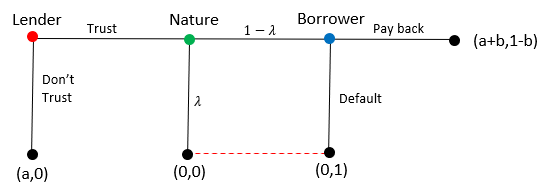
\includegraphics[scale = .8]{figure1.png}
		\end{center}
	
\pagebreak
	\item When $\gamma$ decreases to 1.01, the steady-state values of $K$ and $c$ do not change. This is unsurprising, given that $\gamma$ does not appear in our analytical solution of the steady state. However, the saddle path gets steeper, meaning that one-time shocks will cause a larger change in consumption, and consumption will proceed to move to the steady state more quickly.
		\begin{center}
			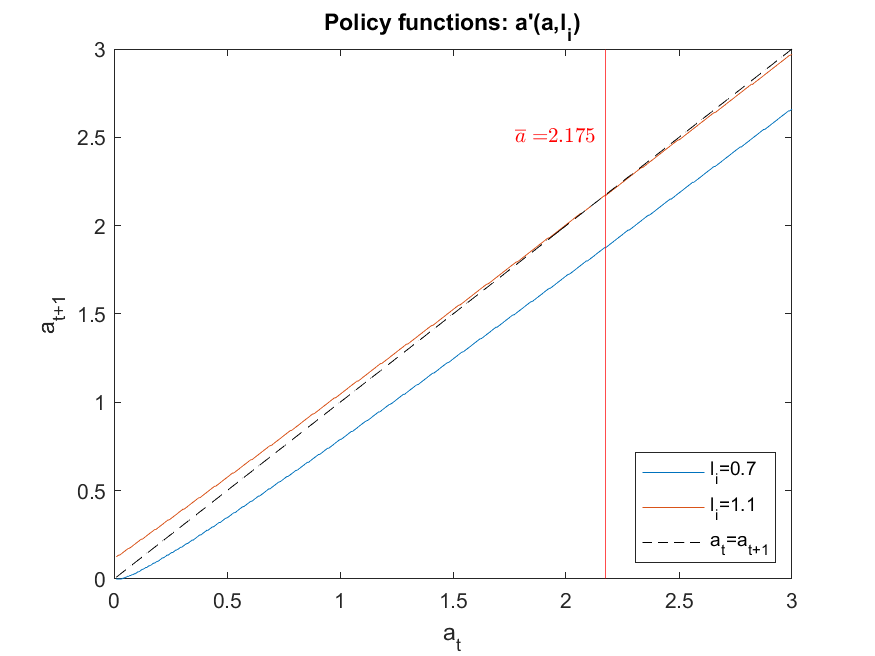
\includegraphics[scale = .8]{figure2.png}
		\end{center}
	
\pagebreak
	\item Productivity, $z$, appears only in the steady-state value of consumption. Thus, a permanent, unexpected shock to productivity will change the steady-state value of consumption, but not that of capital. Since movements along the saddle path to the steady state are achieved by immediate changes to consumption but gradual accumulation or depreciation of capital, this shock to productivity will cause an immediate, one-time increase in consumption that moves the agent from the old steady-state to the new one. This is shown in the plot below.
		\begin{center}
			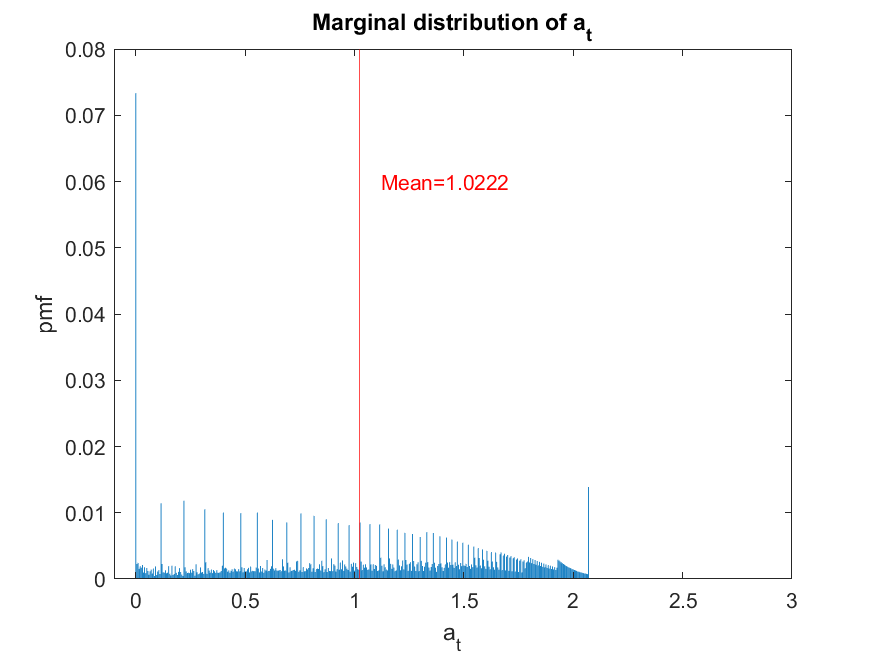
\includegraphics[scale = .8]{figure3.png}
		\end{center}
	
\end{enumerate}

%%%________________________________________________________________%%%


\end{document}












